\subsubsection{Creating the Circular Shift Register}
To create the shift register module press the plus button on the sources window similar to how we added sources previously. However, instead of selecting add file select create file.
\begin{figure}[H]
    \centering
    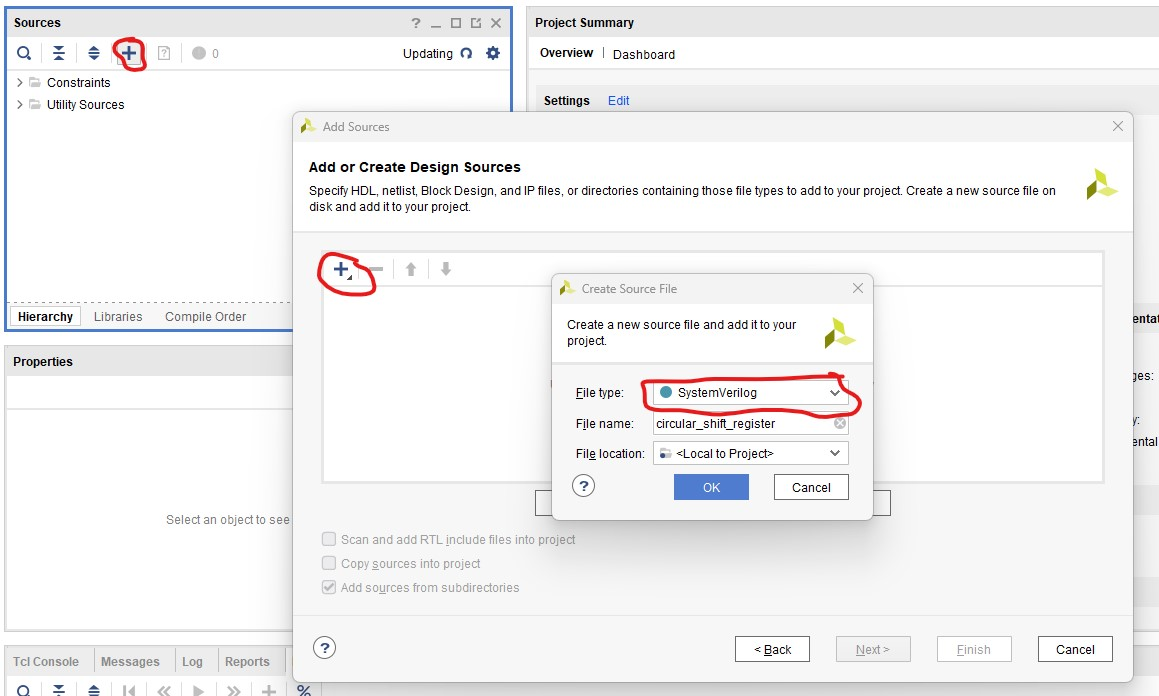
\includegraphics[width=9cm]{Images/CreateFile/create_system_verilog_file.jpg}
    \caption{Create a System Verilog File}
    \label{fig:enter-label}
\end{figure}
\begin{itemize}
    \item Select the Plus in the Sources Window
    \item Select "Add or create design sources"
    \item Select the Plus in the wizard window
    \item Select "Create File..."
    \item Give the file a name: \textit{circular\_shift\_register}. And be sure to select System Verilog.
    \item Select Finish
\end{itemize}
\begin{figure}[H]
    \centering
    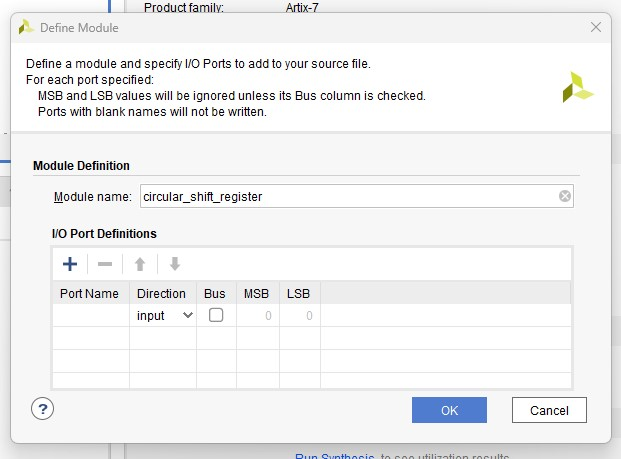
\includegraphics[width=9cm]{Images/CreateFile/DefineModule.jpg}
    \caption{Define Module Window}
    \label{fig:enter-label}
\end{figure}
The define module window will pop up. This defines the input and output ports for the module being designed. Add the ports to the window to produce the following ports. Select bus and adjust MSB to create ports of more than one bit.
\begin{itemize}
    \item Create an input port named clk,
    \item Another Input port named rst\_n,
    \item And finally an output port named reg\_out, make it a bus and make it 128 bits wide (This means the MSB is 127, not 128!)
\end{itemize}
Opening up your module you should see the following:
\begin{verbatim}
    module circular_shift_register(
    input clk,
    input rst_n,
    output [127:0] reg_out
    );
endmodule
\end{verbatim}
The very long register as it is created here will be difficult to work with. Therefore we want to change it to a packed array of 16 8-bit registers. To this end change the register out to be:
\begin{verbatim}
    output logic [7:0] reg_out[15:0]
\end{verbatim}
Now with that setup we can start by declaring the register internally.
\begin{verbatim}
    logic [7:0] circ_reg [15:0];
    assign reg_out = circ_reg;
\end{verbatim}
While we could work directly with the output register instead of having this internal declaration it can be good practice to split it like this as in larger designs it can allow for additional layers of abstraction or for hiding internal states when working with more complicated designs.

\begin{lstlisting}

// Always block triggered by a positive edge of the clock
always_ff @(posedge clk) begin
    if (!rst_n) begin
        // Reset the register array to the initial state
        circ_reg <= ??
|\colorbox{magenta!30}{// Assign appropriate reset values to every element of the circular shift register}|
    end else begin
        // Circularly shift the register array
        circ_reg <= ??
|\colorbox{magenta!30}{// Create the circular shifting register behavior}|
    end
end
\end{lstlisting}

You'll need to create a synchronous reset which will set the value of each 8-bit register in circ\_reg, then on every clock cycle you'll need to create a shift register behavior where the last value in the register becomes the first. Once you believe you have this you'll need to create a new file for the test bench.\\

This module is simple enough that you can practically test every possible state by declaring the device under test, resetting the registers to bring them into known states, and running through the clock 16 times to cycle through all possible values. You can also be much more creative with the test bench if you so choose.

\begin{lstlisting}
module tb_circular_shift_register;

    // Parameters
    parameter WIDTH = 8;
    parameter SIZE = 16;

    // Clock and reset signals
    logic clk;
    logic rst_n;

    // Output array for observing the register state
    logic [WIDTH-1:0] reg_out[SIZE-1:0];

    // Instantiate DUT
    circular_shift_register u_circular_shift_register (
        .clk(clk),
        .rst_n(rst_n),
        .reg_out(reg_out)
    );

    // Clock generation
    always begin
        #5 clk = ~clk; // 10 time unit period
    end

    // Testbench stimulus
    initial begin
        // Initialize signals
        clk = 0;
        rst_n = 0;
        
        // Apply reset
        #10 rst_n = 1;

        // Loop through 16 cycles and print the register state
        repeat (SIZE) begin
            #10; // Wait for one clock cycle
            $display("Register State:");
            $display("reg_out[0] = %h",reg_out[0]) ;
            ... ...
        end

        // Finish the simulation
        $finish;
    end

endmodule
\end{lstlisting}
You can use this to test your circular shift register. You will potentially want to add some additional code to improve the test bench. You can add checks to confirm that it is indeed circling, or you can manually observe the behavior in the waveform window. 